\section{Sejarah Android Studio}
	Pertama kali muncul Android Inc merupakan sebuah perusahaan software kecil yang didirikan pada bulan Oktober 2003 di Palo Alto, California, USA. Perusahaan ini dibangun oleh beberapa senior di beberpa perusahaan yang berbasis IT dan Communication, Andy Rubin, Rich Miner, Nick Sears dan Chris White.
Rubin menyatakan bahwa, Android Inc Didirikan untuk mewujudkan mobile device yang lebih fleksibel terhadap lokasi dan preferensi pemilik. Sehingga, Android Inc ingin mewujudkan mobile device yang lebih mengerti pemiliknya selain karena OS nya yang open source.

Berawal dari konsepan inilah Android Inc ternyata menarik minat Google untuk memilikinya. Maka, pada bulan Agustus 2005, Akhirnya Android Inc diakuisisi oleh Google Inc. dan seluruh sahamnya dibeli oleh Google.
Perusahaan milik Andy Rubin, Rich Miner, Nick Sears dan Chris White tetap di Android Inc yang dibeli Google, sehingga akhirnya mereka pun ikut  menjadi bagian dari raksasa Google dan sejarah Android. Disini mereka mulai menggunakan platform Linux untuk membuat sistem operasi bagi mobile phone.

Dari sinilah akhirnya banyak pengembang sistem maupun software yang mengembangkan maupun merancang sistem Android menggunakan software – software yang support dengan Android, Contohnya ialah : Android Studio.
\section{Definisi Android Studio}
Android Studio adalah Lingkungan Pengembangan Terpadu (Integrated Development Environment/IDE) resmi untuk pengembangan aplikasi Android, yang didasarkan pada InelliJ IDEA. Selain sebagai editor kode dan fitur developer IntelliJ yang andal, Android Studio menawarkan banyak fitur yang meningkatkan produktivitas Anda dalam membuat aplikasi Android, seperti: 
\begin{enumerate}
\item Sistem build berbasis Gradle yang fleksibel.
\item Emulator yang cepat dan kaya fitur.
\item Lingkungan terpadu tempat Anda bisa mengembangkan aplikasi untuk semua perangkat Android.
\item Terapkan Perubahan untuk melakukan push pada perubahan kode dan resource ke aplikasi yang sedang berjalan tanpa memulai ulang aplikasi.
\item Template kode dan integrasi GitHub untuk membantu Anda membuat fitur aplikasi umum dan mengimpor kode sampel.
\item Framework dan fitur pengujian yang lengkap.
\item Fitur lint untuk merekam performa, kegunaan, kompatibilitas versi, dan masalah lainnya.
\item Dukungan C++ dan NDK.
\item Dukungan bawaan untuk Google Cloud Platform, yang memudahkan integrasi Google Cloud Messaging dan App Engine.
\end{enumerate}

\section{Macam-Macam Android Studio }
\begin{enumerate}
\item Android 1.0 (Apple Pie)Android versi pertama ini dirilis pada 23 September 2008 dan hanya dilengkapi fitur-fitur seperti Play Store, Web Browser, Kamera, Sinkronisasi antara Gmail, Contacts dan Google Agenda. Selain itu, diawal perilisannya, Android juga sudah dilengkapi aplikasi Google Maps serta dukungan streaming Youtube.
\item Android 1.1 (Banana Bread)Sistem Operasi android yang rilis selanjutnya adalah Banana Bread, rilis pada bulan Februari 2009. Dan fitur ini juga tidak jauh berbeda dengan versi sebelumnya.
HTC adalah salah satu ponsel Android pertama yang menggunakan versi ini.
\item Android 1.5 (Cupcake)Rilis pada awal bulan April 2009 dan juga tidak jauh berbeda dengan versi Android sebelumnya. Hanya saja ada fitur tambahan seperti Support Bluetooth A2DP, AVRCP, Soft-keyboard dengan prediksi text dan record/watch videos.
\item Android 1.6 (Donut)Android Donut rilis pada 15 September 2009, dan mendapat fitur tambahan seperti Gesture Framework hingga Turn-by-turn navigation. Selain itu, Android ini juga terlihat lebih sempurna pada waktu itu. Dengan minimnya bug, ditambah lebih lengkapnya fitur-fitur yang disediakan Google.
\item Android 2.0 (Éclair)Android versi 2.0 bernamakan Eclair dan rilis pada 26 Oktober 2009 silam. Yang selain bluetooth, Android versi ini juga mendapatkan fitur multi-touch, Live Wallpaper dan juga flash kamera.
Selain itu, adapun beberapa fitur yang dapat anda nikmati dalam Android versi ini adalah yakni, HTML, Digital zoom, Support Microsoft Exchange, dan Updated UI.
\item Android 2.2 9 (Froyo)Pada bulan Mei 2010 lalu, Google telah merilis Android versi terbaru pada waktu itu. Yakni adalah Android 2.2 9 (Froyo). Versi ini merupakan salah satu sistem operasi Android yang juga telah disempurnakan, utamanya tentu untuk meningkatkan kecepatan kinerja suatu Android.
Dan berikut ini adalah fitur dan perbaikan yang disediakan oleh Android versi 2.2 9 :
\begin{enumerate}
\item Peningkatan Speed
\item Implementasi JIT
\item USB Tethering
\item Aplikasi instalasi untuk perluasan memori
\item Support file upload pada the browser
\item Animated GIFs
\end{enumerate}
\item Android 2.3 (Gingerbread)
Pada bulan Desember 2010 lalu, Google secara resmi merilis Android versi terbaru, Gingerbread. Yang secara fitur jelas sudah sangat sempurna. Ditambah lagi, Android versi 2.3 ini juga diadopsi oleh salah satu perusahaan Smartphone paling terkenal, yaitu Samsung dengan menanamkan sistem operasi ini dalam ponsel seri Nexus-nya.
\item Android 3.0 – 3.2.6 (Honeycomb)
Honeycomb merupakan salah satu sistem operasi Android versi terbaru yang rilis pada bulan Februari 2011 silam. Namun, versi ini lebih ditujukkan untuk Tablet yang mana pada tahun itu sangat laris dipasaran.
Fitur dan perbaikan pada Android versi ini:
\begin{enumerate}
\item Support Multi core
\item Support Tablet lebih baik
\item Updated 3D UI
\item Layar Utama (homescreens) yang bisa diatur
\item Melihat aplikasi yang barusan dibuka
\item Menyempurnakan layout keyboard
\item Transport protocol untuk Media/Picture
\item video chat Google Talk
\item Google eBooks
\item “Private browsing”
\item System-wide Clipboard
\item HTTP Live streaming
\end{enumerate}
\subsection{Update 3.1}
\begin{enumerate}
\item Peningkatan UI
\item Open Accessory 
\item USB host API
\item Support mouse, joysticks dan gamepad
\item Notificasi MTP
\item RTP API untuk audio
\end{enumerate}
\subsection{Update 3.2}
\begin{enumerate}
\item Optimise untuk berbagai tablets
\item Mode kompatibilitas display  (zoom for fixed-sized apps)
\item Sinkronisasi Media dari SD card
\end{enumerate}
\subsubsection{Update 3.2.1}
\begin{enumerate}
\item Update Android Market termasuk automatic updates yang lebih mudah
\item Update Google Books
\item Peningkatan kinerja Wi-Fi
\item Perbaikan prediksi tulisan tangan huruf Chinese
\end{enumerate}
\subsubsection{Update 3.2.2}
\begin{enumerate}
\item Perbaikan kecil
\end{enumerate}
\subsubsection{3.2.4}
\begin{enumerate}
\item Update tambahan ‘Pay as you go’ untuk tablet
\end{enumerate}
\subsubsection{Update 3.2.6}
\begin{enumerate}
\item Perbaikan kecil
\end{enumerate}
\item Android 4.0 (Ice Cream Sandwich )Puncak kematangan Android yakni ketika pada versi ini, yang mana Ice Cream Sandwich rilis pada bulan Oktober 2011 silam. Dan operasi sistem ini mulai bekerja di semua jenis smartphone apapun. Selain bertambahnya fitur-fitur menarik, Ice Cream Sandwich juga merupakan versi Android paling banyak disukai pada waktu itu. Bahkan, Android Ice Cream Sandwich juga dilengkapi dengan fitur ekstra multitasking dan notifikasi yang lebih banyak.
\item Android 4.1.2 (Jelly Bena)
Jelly Bean rilis pada 9 Juli 2012 lewat konferensi I/O Google. Versi ini merupakan salah satu versi Android yang kerap mendapatkan update fitur-fitur yang berguna dan menarik, beberapa halnya adalah seperti memperbaiki rotasi layar, seperti Support resolusi video 4K, Support penulisan huruf Hebrew and Arabic dari kanan ke kiri, dan peningkatan kinerja, sistem keamanan dan masih banyak lainnya.
\item Android 4.4 (Kitkat)
Android versi inilah yang saat ini banyak digunakan oleh mayoritas masyarakat Indonesia. Kitkat adalah versi Android yang rilis pada 2013 lalu. pada versi ini, Android banyak mendapatkan pembaharuan fitur. Seperti, terdapat fitur Screen recording, untuk merekam kegiatan yang terjadi pada layar smartphone anda, New Translucent system UI, Peningkatan akses notifikasi, System-wide settings untuk closed captioning, Peningkatan kinerja dan masih banyak yang lainnya.
\item Android 5.0 (Lollipop)Rilis pada tahun 2014, Android yang satu ini lebih banyak menawarkan fitur tambahan untuk menyempurnakan fitur-fitur yang sudah ada. Dan Nexus 6 adalah salah satu ponsel yang paling pertama mencicipi Android versi ini. Selain itu, Google juga lebih menyempurnakan kinerja dari Android Lollipop sendiri
\item Android 6.0 (Marshmallow)Android versi 6.0 merupakan salah satu sistem operasi Android yang rilis pada tahun 2015 silam, yang mana banyak membawa pembaharuan. Salah satunya adalah support USB Type-C. Tidak hanya itu saja, Android versi 6 ini serta memberikan fasilitas autentikasi sidik jari dan daya baterai yang lebih meningkat
\item Android 7.0 (Nougat)Android Nougat versi 7.0 rilis pada bulan Agustus 2016 silam yang lebih meningkatkan kinerja versi Android sebelumnya. Selain itu, Android Nougat juga mendapatkan banyak fitur-fitur baru yang diantaranya seperti dapat multitasking,  meningkatkan fitur Doze yang dulu telah rilis di Android versi sebelumnya.
Dan inilah beberapa fitur terbaru yang terdapat pada Nougat.
\begin{enumerate}
\item Support Multi window
\item Dapat langsung membalas pesan dari jendela atau menu notifikasi.
\item Tampilan panel notifikasi dan quick settings yang baru.
\item Mode Doze yang ditingkatkan, (Doze Mode 2.0)
\item Menu di antara system settings.
\end{enumerate}
\item Android 8.0 ( Oreo)Android versi Oreo rilis pada bulan Agustus 2017 lalu. Tentu saja Android versi ini adalah versi final untuk sekarang ini. Beberapa fitur juga turut diluncurkan Google selaku pihak pengelola. Adapun fitur-fitur tersebut antara lain adalah
\begin{enumerate}
\item Android O lebih fokus pada kecepatan dan efisiensi
\item Kecepatan Boot up 2X lebih cepat
\item Mode Picture in picture lebih flexibel dari Android N
\item Aplikasi yang berjalan di latarbelakang lebih diperketat untuk menghemat battery
\item Battery lebih tahan lama
\item Emoji yang diperbaharui dan lebih banyak
\end{enumerate}
\section{Karakteristik Android Studio}
\begin{enumerate}
\item Terbuka
\hfill \break
Android dibangun untuk benar-benar terbuka sehingga sebuah aplikasi dapat memanggil salah satu fungsi inti ponsel seperti membuat panggilan, mengirim pesan teks, menggunakan kamera dan lain-lain. Android merupakan open source, dapat secara bebas diperluas untuk memasukkan teknologi baru yang lebih maju pada saat teknologi tersebut muncul.
\item Semua aplikasi dibuat sama
\hfill \break
Android tidak memberikan perbedaan terhadap aplikasi utama dari telepon dan aplikasi pihak ketiha(third-party application). Semua aplikasi dapat dibangun untuk memilih akses yang sama terhadap kemampuan sebuah telepon dalam menyediakan layanan dan aplikasi yang luas terhadap para pengguna.
\item Memecahkan hambatan pada aplikasi
\hfill \break
Android memecah hambatan untuk membangun aplikasi yang baru dan inovatif. Misalnya, pengembang dapat menggabungkan informasi yang diperoleh dari web dengan data pada ponsel seseorang seperti kontak pengguna,kalender atau lokasi geografis.
\item Pengembangan aplikasi yang cepat dan mudah
\hfill \break
Android menyediakan akses yang sangat luas kepada pengguna untuk menggunakan aplikasi yang semakin baik. Android memiliki sekumpulan tools yang dapat digunakan sehingga membantu para pengembang dalam meningkatkan produktivitas pada saat membangun aplikasi yang dibuat.
\end{enumerate}
\section{Varian Build}
\hfill \break
Sistem build dapat membantu teman-teman untuk membuat beberapa versi berbeda untuk aplikasi yang sama dari satu project. Hal ini berguna saat Anda menyediakan aplikasi dalam versi gratis dan berbayar, atau jika teman-teman ingin mendistribusikan beberapa APK untuk berbagai konfigurasi perangkat di Google Play.
\section{Fitur Profil dan Debug}
\hfill \break
Gunakan proses debug inline untuk menyempurnakan panduan kode Anda dalam tampilan debugger verifikasi inline untuk referensi, ekspresi, dan nilai variabel. Informasi debug inline meliputi :
\begin{enumerate}
\item Nilai variabel inline
\item Objek perujuk yang merujuk ke objek terpilih
\item Nilai yang dihasilkan metode
\item Ekspresi operator dan lambda
\item Nilai tooltip
\end{enumerate}
\section{Pesan Log}
\hfill \break
Saat membuat dan menjalankan aplikasi dengan Android Studio, Anda bisa melihat output pada adb dan pesan log perangkat di jendela Logcat.
\section{Manfaat Mempelajari Android Studio}
\begin{enumerate}
\item Dengan mempelajari Android Studio dapat membantu Anda untuk mempercepat pembuatan Aplikasi yang Anda Inginkan
\item Android Studio merupakan sebuah tools yang mudah dipahami dan digunakan
\item Dalam satu tools ini Anda bida mendapatkan berbagai manfaat mulai dari pembuatan aplikasi hingga testing aplikasi
\item Bahkan, dengan belajar Android Studio maka Anda bisa menghemat waktu kerja untuk dapat lebih priduktif
\item Dapat memperdalam ilmu codingan dengan baik. Karena dalam android studio diberikan beberapa refensi ketika mengetik sintaks. Dengam begitu tentunya Anda akan mencari tahu apa saja kegunaan dari sintaks yang terdapat.
\item Sarana pembelajaran coding dan pembuatan aplikasi yang baik dan praktis hanya dengan Android Studio.
\end{enumerate}
\end{enumerate}
\section{Antarmuka Pengguna}
\hfill \break
Jendela utama Android Studio terdiri dari beberapa area logis yang diidentifikasi dalam gambar seperti di bawah ini :
\begin{figure}[!htbp]
  \centering
  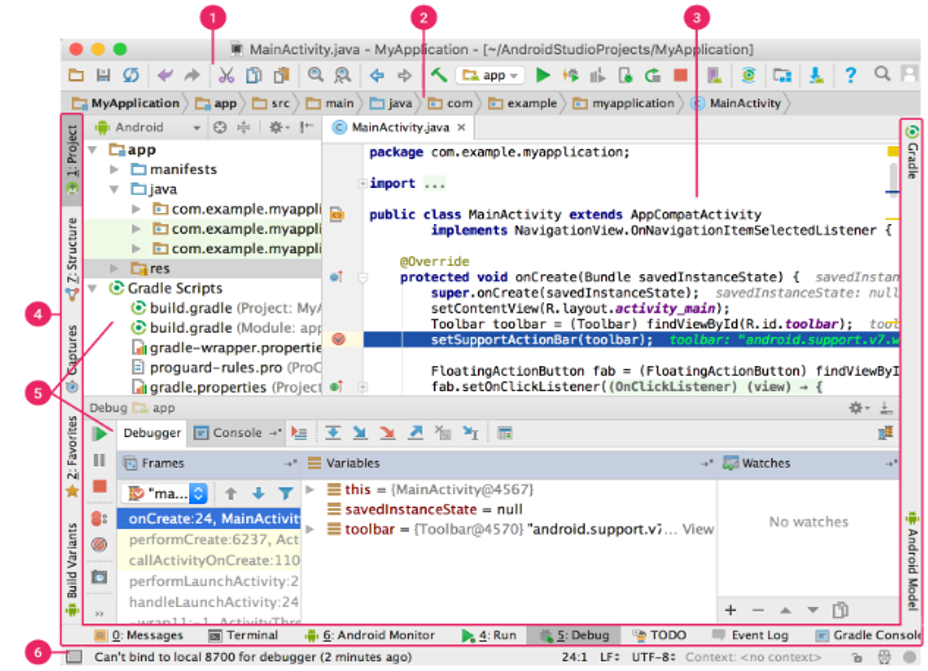
\includegraphics[width=.75\textwidth]{figures/JU.png}
  \caption{Jendela Utama Android Studio}\label{fig:error}
\end{figure}
\begin{enumerate}
\item Toolbar
\hfill \break
Toolbar memungkinkan Anda melakukan berbagai tindakan, termasuk menjalankan aplikasi dan meluncurkan fitur Android
\item Menu Navigasi
\hfill \break
Menu navigasi membnatu Anda menjelajah project dan membuka file untuk di edit. Menu ini memberikan tampilan struktur yang lebih ringkas yang terlihat di jendela Project.
\item Jendela Editor
\hfill \break
Jendela Editor adalah tempat Anda membuat dan memodifikasi kode. Tergantung jenis file yang ada, editor ini dapat berubah. Misalnya, saat menampilkan file tata letak, editor akan menampilkan Layout Editor.
\item Panel Jendela Fitur
\hfill \break
Panel Jendela Fitur berada di sisi luar jendela IDE dan berisi tombol-tombol yang memungkinkan Anda memperluas atau menciutkan setiap jendela fitur.
\item Jendela Fitur
\hfill \break
Jendela Fitur memberi Anda akses ke tugas tertentu seperti pengelolaan project, penelusuran, kontrol versi dan banyak lagi. Anda dapat memperluas dan menciutkan jendela ini.
\item Status Bar
\hfill \break
Status Bar menampilkan status project Anda dan IDE itu sendiri, serta semua peringatan atau pesa.
\end{enumerate}
\section{Bahasa Java}
\hfill \break
Bahasa Pemrograman Java
\begin{figure}[!htbp]
  \centering
  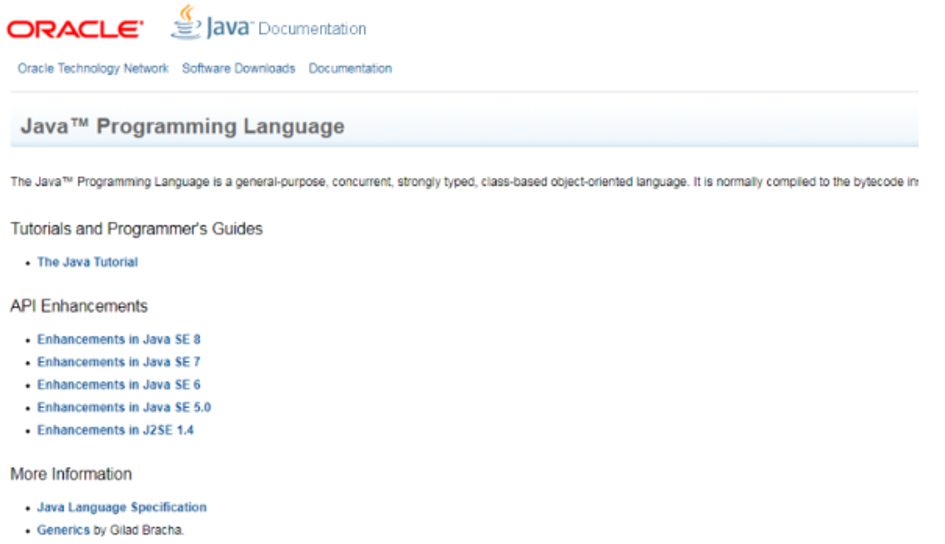
\includegraphics[width=.75\textwidth]{figures/java.png}
  \caption{Bahasa pemrograman yang digunakan untuk menbuat aplikasi ini adalah bahasa Java}\label{fig:error}
\end{figure}
\hfill \break
Bahasa pemrograman java merupakan bahasa yang berada pada urutan 10 besar bahasa pemrograman yang terpopuler di dunia saat ini. Bahasa pemrograman Java pada tahun 2017 merupakan bahasa paling populer, namum sekarang sudah disalip oleh bahasa pemrograman JavaScript dan Python.
\hfill \break
Salah satu penyebabnya yaitu karena jutaan aplikasi android dibuat menggunakan bahasa pemrograman java. Untuk membuat aplikasi android menggunakan bahasa java kita bisa menggunakan tools atau IDE:
\begin{enumerate}
\item Android Studio (IDE resmi didukung penuh oleh google)
\item Eclipse (IDE lain yang sebelumnya didukung penuh oleh google sebelum adanya android studio)
\end{enumerate}
\hfill \break
Untuk pemula yang baru ingin membuat aplikasi android disarankan menggunakan bahasa pemrograman java.
\section{Bahasa Kotlin}
\hfill \break
Bahasa Pemrograman Kotlin
\begin{figure}[!htbp]
  \centering
  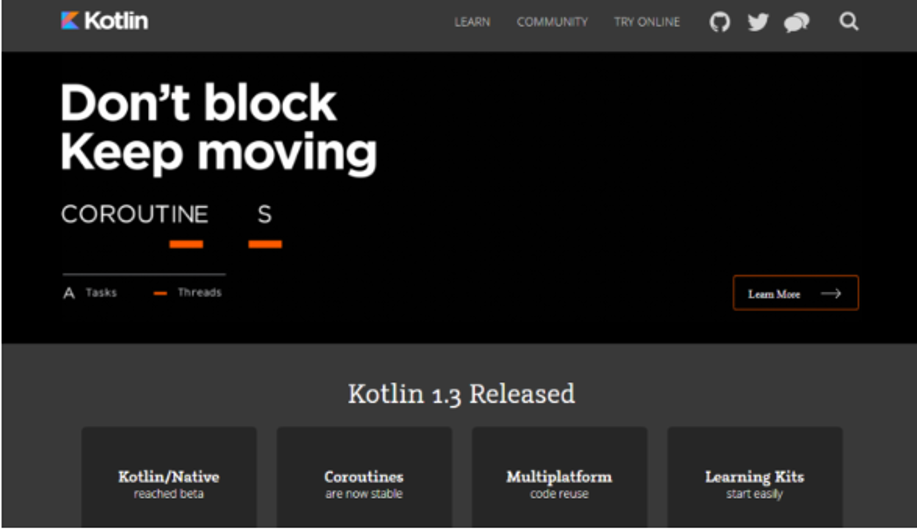
\includegraphics[width=.75\textwidth]{figures/Kotlin.png}
  \caption{Bahasa pemrograman yang digunakan untuk menbuat aplikasi pada android Studio bisa juga menggunakan bahasa kotlin}\label{fig:error}
\end{figure}
\hfill \break
Kotlin dicipyakan oleh JetBrains yaitu perusahaan yang terkenal membuat IDE seperti : Android Studio, RubbyMine,PHPStrome, dll.
\hfill \break
Kotlin sengaja diciptakan oleh JetBrains untuk melengkapi segala kekurangan dari bahasa pemrograman Java. Memang benar bahasa pemrograman kotlin lebih simple dibandingkan Java.
\hfill \break
Keunggulan lainnya dari bahasa Kotlin yaitu bahasa ini bisa berjalan beriringan dengan bahasa pemrograman Java. Dan juga bisa menggunakan library dari Java.
\hfill \break
Pembuatan aplikasi android saat ini bisa menggunakan IDE :
\begin{enumerate}
\item Intellij IDEA
\item Android Studio
\item Eclipse
\end{enumerate}